\documentclass[a4j,12pt]{jreport}
\usepackage[dvipdfmx]{graphicx}
\usepackage{mythesis}
\usepackage{multirow}
\usepackage{here}
\usepackage{url}
\usepackage{comment}
\setlength{\itemsep}{-1zh}
\title{}
\icon{
		
\includegraphics[width=80mm,bb=0 0 595 842]{fig/ryukyu.pdf}
	}
\year{平成26年度 卒業論文}
\belongto{琉球大学工学部情報工学科}
\author{115702H 新里亮太 \\ 指導教員 宮里智樹 }
%%
%% プリアンブルに記述
%% Figure 環境中で Table 環境の見出しを表示・カウンタの操作に必要
%%
\makeatletter
\newcommand{\figcaption}[1]{\def\@captype{figure}\caption{#1}}
\newcommand{\tblcaption}[1]{\def\@captype{table}\caption{#1}}
\makeatother
\setlength\abovecaptionskip{0pt}

\begin{document}

% タイトル
\maketitle
\baselineskip 17pt plus 1pt minus 1pt

\pagenumbering{roman}
\setcounter{page}{0}

\tableofcontents	% 目次
\listoffigures		% 図目次
\listoftables		% 表目次

%以下のように、章ごとに個別の tex ファイルを作成して、
% main.tex をコンパイルして確認する。
%章分けは個人で違うので下のフォーマットを参考にして下さい。

%はじめに
\chapter{はじめに}
\label{chap:introduction}
\pagenumbering{arabic}

\section{背景}
日本では,高齢者人口が増加し少子高齢化社会が加速している.
それに伴い,増加しているのが認知症患者数である.
厚生労働省の調査\cite{厚生労働省}によると2010年時点で200万人程度といわれ,専門家の間では,すでに65歳以上人口の10\%(242万人程度)に達しているという意見もある.

年々増加している認知症患者であるが,介護現場では,徘徊による事故を防止するために,家族や介護者が多大な負担を強いられているのが現状である.
認知症患者の介護者への調査\cite{山梨県}によると,見守りが常に必要な割合が4割にものぼり,徘徊などで行方不明になったとして警察に届けられている数は9607人に及ぶ.
愛知県大府市で2007年12月,徘徊症状がある認知症の男性が電車にはねられるという事故が発生し,介護者である男性の遺族への賠償判決が出された.

これらの現状から,介護者の負担を軽減し,認知症患者の徘徊を防止する仕組みの構築は急務だといえる.
介護者への負担軽減を目的とした電子的・機械的なセンサーシステムはすでにあるが,既存施設への電気設備の敷設が困難,外出先での対応ができないなどの課題がある.
そのため,スマートフォンを受信機とし,低価格の発信機(iBeacon)を利用した電子見守りシステムの構築を株式会社国建システムと共同で行う.

電子見守りシステムでは、発信機と受信用スマートフォンが、1対1,1対多,多対多の組み合わせでの見守りが可能なしくみを開発する.
特に受信用スマートフォンが複数ある場合,スマートフォン同士でアドホックネットワークを構築し,発信機の情報を共有することで見守りエリアの拡大を図る.

\section{研究目的}
本研究では,上述の電子見守りシステムのスマートフォン同士のアドホックネットワークの構築と,情報共有手法の実装を行い,それらの検討を行う.
電子見守りシステムでは介護者それぞれのスマートフォンを用いて見守りを行うことを想定しており,異なる機器やOSでの開発が予想される.
そのため,クロスプラットフォームなP2P(peer-to-peer)型端末通信フレームワークであるAllJoynを用いてアドホックネットワークの構築を行う.

\section{本論文の構成}
本論文の構成について解説する.

本章では,「はじめに」として本研究の背景と目的について述べた.
第二章では,本研究に関する概念や技術について述べる.
第三章では,本研究の背景としてある電子見守りシステムについて述べる.
第四章では,本研究で作成したアプリケーションの設計や仕様,考察にいて述べる.
第五章では,今後の課題について述べる.
%\section{Introduction}


%基礎概念
\chapter{基礎概念}
\label{chap:concept}

\section{アドホックネットワーク}
アドホックネットワーク\cite{アドホック}とは,アクセスポイントを必要としない無線で接続できる端末のみで構成されたネットワークである.
直接電波が届き通信可能である場合には,始点端末から終点端末へ1ホップでパケット伝達が行われる.
電波が直接届かない場合には経由(マルチホップ)することで終点端末までパケットを伝達する.
端末の中継機能を利用してネットワークを構成しているので,アドホックネットワークには基地局インフラが不要である.
そのため、限られた領域内の簡易なネットワークの構築の手段として有効である.

以下の図では始点端末から終点端末まで直接繋がっていないが,他の端末を経由し4ホップで通信を行っている.

\begin{figure}[htbp]
\centering
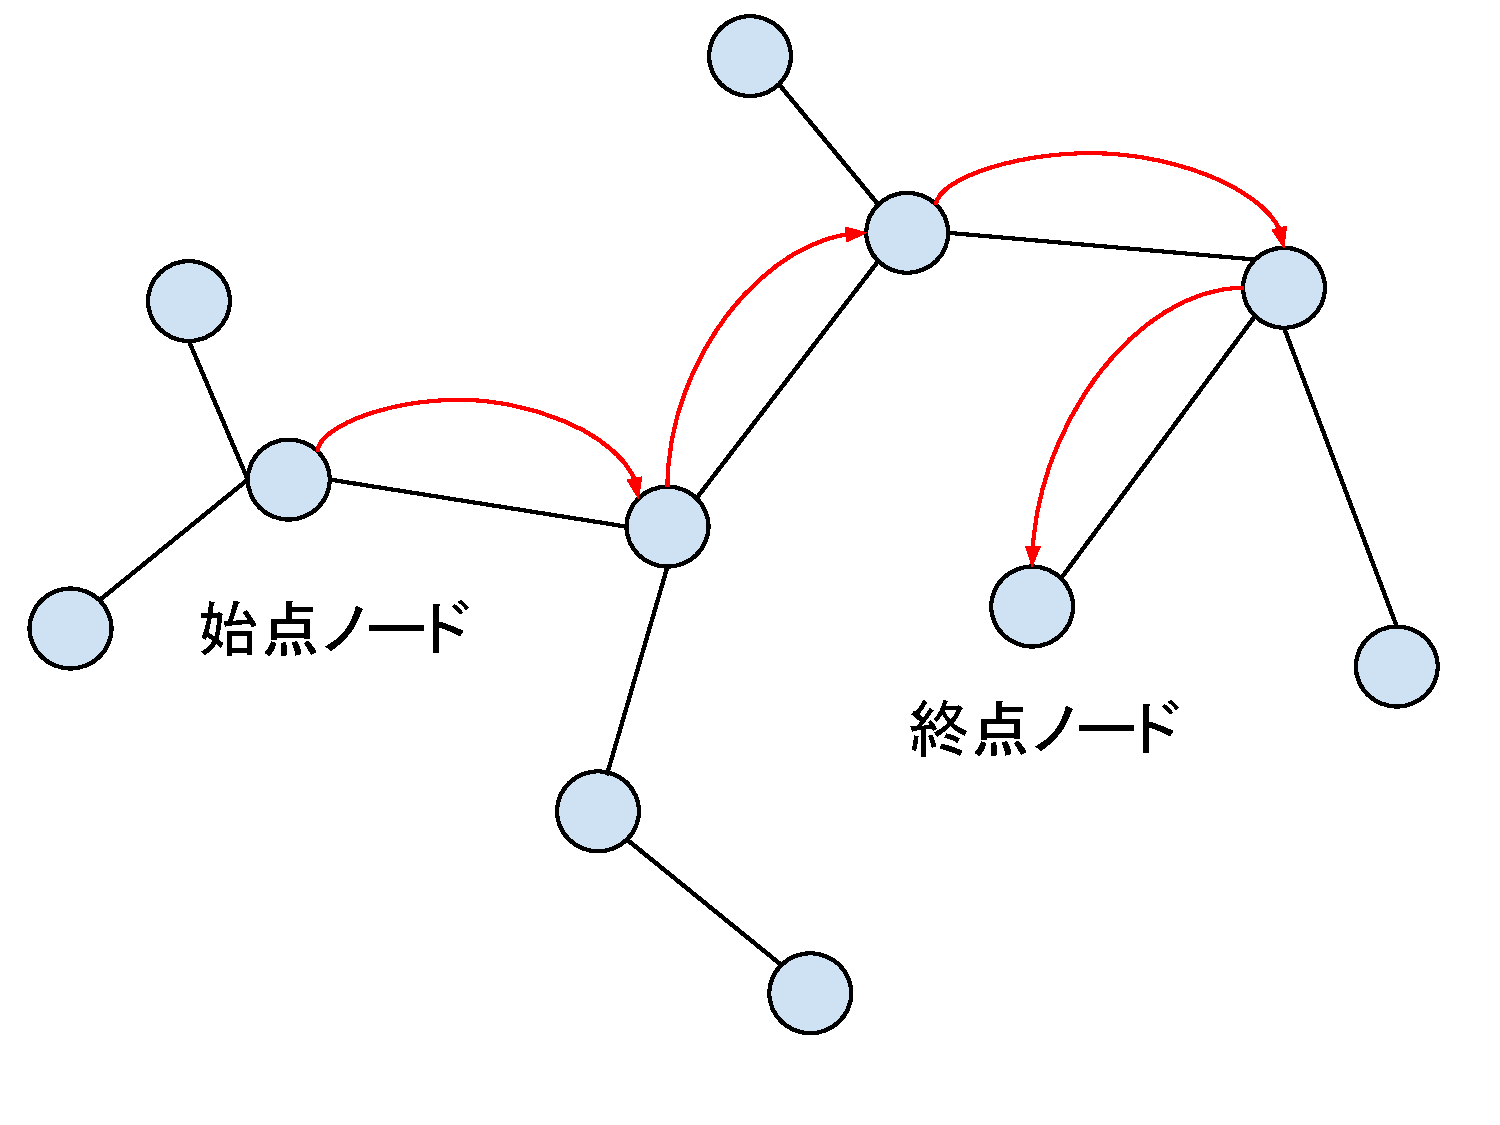
\includegraphics[width=10cm]{fig/ad-hoc.pdf}
\caption{アドホックネットワークの例}
\end{figure}

\section{AllJoyn}
AllJoyn\cite{allseen}\cite{スライド}はQualcommが開発したオープンソースプロジェクトである.
端末間通信を実現し,製品やアプリケーション間の相互運用を可能にするデバイス通信フレームワークを提供している.
QualcommはloT標準化団体であるAllSeenに参加しており,AllSeenが推進するloT規格はAllJoynをベースに設計されている.
OSI参照モデルのセッション層以上の規格であり,トランスポート層には依存しないというメリットがある.
そのため,Wi-FiやWi-Fi Direct,Bluetoothといった様々な通信規格を用いて開発することができる.
Android,iOS,OS X,Linux,Windows7など様々なOSに対応し,Java,C++,C,JavaScriptなどの言語で使用できる.
AllJoynは近傍デバイスの探索やP2Pネットワークへの接続,セキュリティなどの要素を提供しており,機器やOSに依存せず開発することができる.

\begin{figure}[htbp]
\centering
\includegraphics[width=10cm]{fig/AllJoyn_App.pdf}
\caption{AllJoynを用いたアプリケーションの例}
\end{figure}

\subsection{AllJoynアーキテクチャ}

AllJoynネットワークはAllJoynアプリケーションとAllJoynルーターから成る.
AllJoynアプリケーションはAllJoynルーターを通じて他のAllJoynアプリケーションやAllJoynルーターと通信を行う.
AllJoynアプリケーションは以下の要素から成る.

\begin{itemize}
\item AllJoyn App Cods
\item AllJoyn Service Frameworks Libraries
\item AllJoyn Core Library
\end{itemize}

\begin{figure}[htbp]
\centering
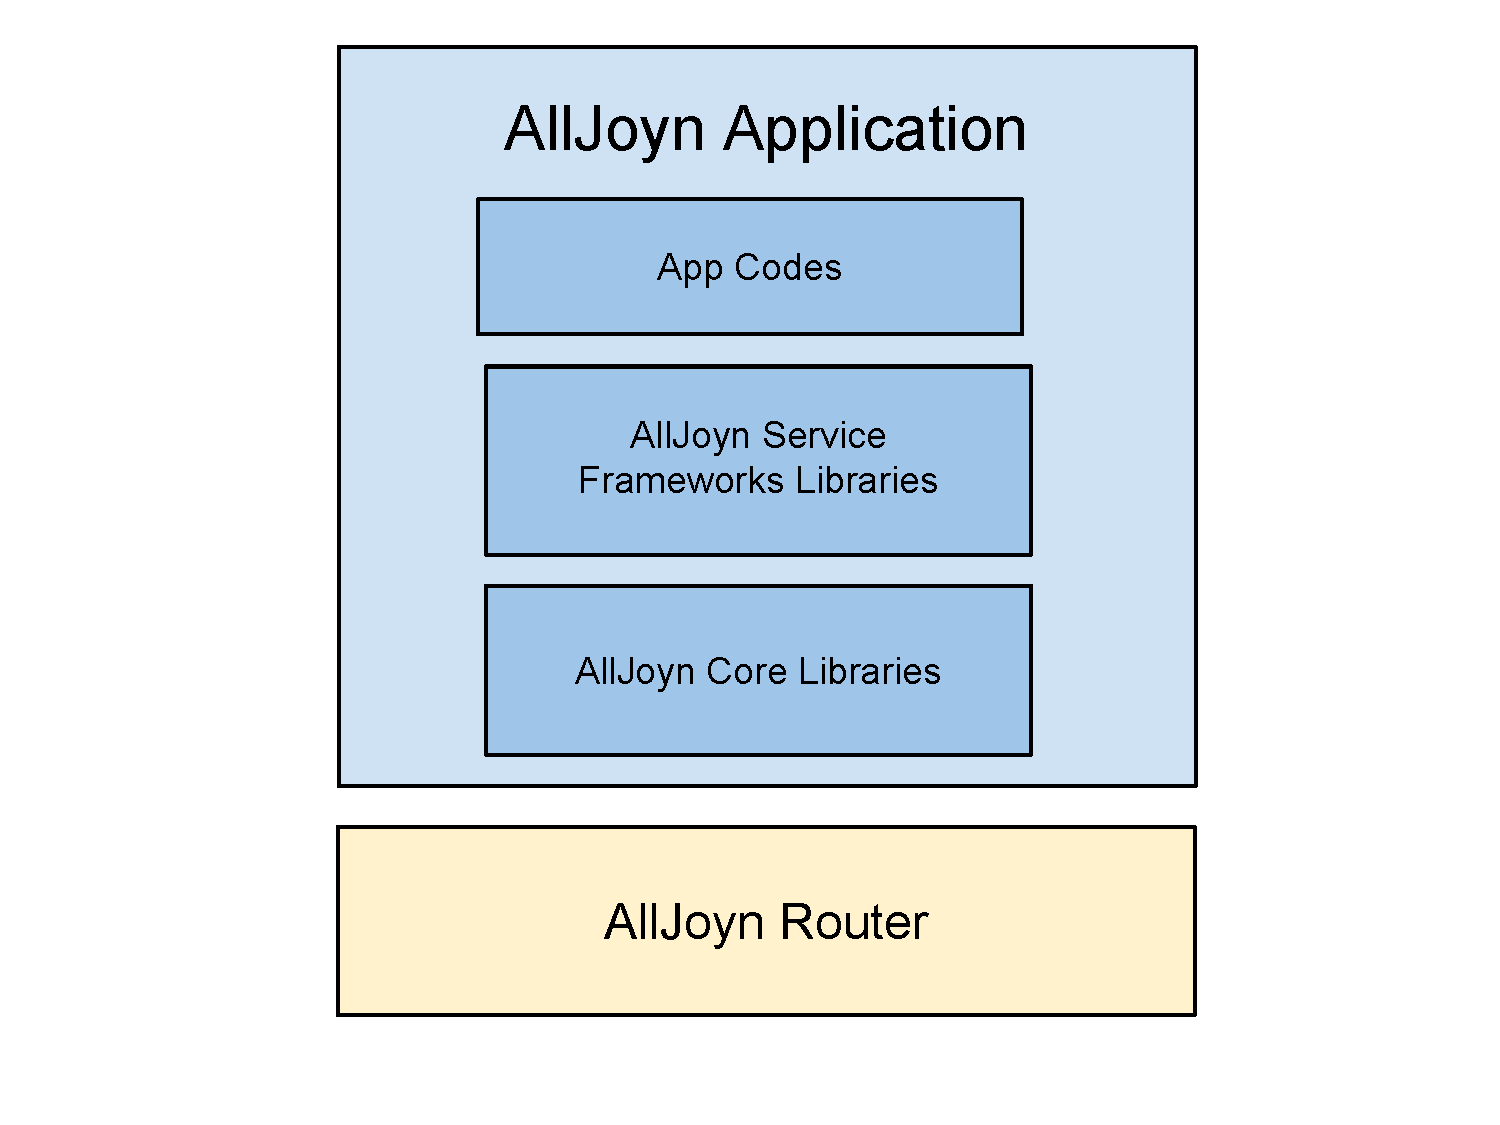
\includegraphics[width=10cm]{fig/AllJoyn.pdf}
\caption{AllJoynアーキテクチャの構成}
\end{figure}

\subsubsection{AllJoyn Core Library}
AllJoyn Core LibraryはAllJoynネットワークと通信するための最低限のAPIを提供する.
提供するAPIは以下の通りである.

\begin{itemize}
\item Advertisement \\
UDPパケットを用いてAllJoynサービスをブロードキャストする.
\item Discovery \\
AdvertisementされたAllJoynサービスを検索する.
\item Session creation \\
セッションの確立
\item Interface definition of methods, properties, and signals \\
メソッド,プロパティ,シグナルのインターフェース定義
\item Object creation and handling \\
オブジェクトの生成とハンドリング
\end{itemize}

\subsubsection{AllJoyn Service Framework Libraries}
AllJoyn Service Framework Librariesは,onboarding,notificatino,control panelなどのサービスを備えている.
Base Servicesとして以下の機能がある.

\begin{itemize}
\item Base Services
\begin{itemize}
\item Onbording \\
Wi-Fiネットワークへの接続をサポート
\item Configuration \\
端末の構成
\item Notificatinos \\
デバイスからの通知
\item Control Panel \\
UI widgetとリモート端末との通信
\end{itemize}
\end{itemize}

AllJoyn Service Framework Librariesを使うことで,アプリケーションや端末は互いにこれらのサービスを運用することができる.


\subsubsection{AllJoyn App Code}
AllJoyn App CodeはAllJoynアプリケーションのロジックである.
高レベルの機能を提供するAllJoyn Service Frameworksか,直接AllJoyn Core APIにアクセスできるAllJoyn Core Libraryのどちらかを用いてプログラミングされる.

\subsubsection{AllJoyn Router}
AllJoyn RouterはP2P Advertisement/Discovery,Connection ManagementといったAllJoynシステムの核となる機能を提供する.
メッセージはAllJoyn Routerを経由して他のアプリケーションに送信される.



\section{Bluetooth Low Energy}
Bluetooth Low Energy(BLE)\cite{BLE1}\cite{BLE2}近距離無線通信技術Bluetoothの拡張仕様の1つであり,Bluetooth4.0規格の一部として採用された.
一般的なBluetoohと同様に2.4GHz帯を使用し,データ転送速度は1Mbpsである.
非常に少ない消費電力で動作することができ,ボタン電池で数年動作すると言われている.

\section{iBeacon}
iBeacon\cite{iBeacon}\cite{iBeaconを使用してみよう}は,2013年にAppleが発表したBluetooth Low Energy(BLE)を利用した技術であり,発信機から発せられるビーコンを受信し,発信機の位置を特定・確認できる.
iOS7以降の端末(iPhone,iPad,およびiPod touch)やAndroid4.3以降の端末などで受信することができる.
iBeaconでは領域の出入りをチェックするリージョン監視やビーコンの情報を受信するレーシングを用いて位置や近接具合などを検知する.
ビーコンを受信したときに得られる情報には以下の6つがある.


\begin{comment}%コメントアウト

\begin{table}[htb]
\centering
\begin{tabular}{|l|l|}  \hline
proximityUUID & 識別子 \\ \hline
major & 識別子 \\  \hline
minor & 識別子 \\ \hline
proximity & ビーコンとの距離 \\ \hline
accuracy & 距離の精度 \\ \hline
RSSI & 受信強度 \\ \hline
\end{tabular}
\end{table}

\end{comment}

\begin{itemize}
\item proximity UUID:ビーコン識別子
\item major:ビーコン識別子
\item minor:ビーコン識別子
\item proximity:ビーコンとの距離
\item accuracy:距離の精度
\item rssi:受信強度
\end{itemize}

また,proximityは正確な距離を表すものではなく,以下の大まかな4つの値で得ることができる.

\begin{comment}%コメントアウト

\begin{table}[htb]
\centering
\begin{tabular}{|l|l|} \hline
Unknown & 検出不可 \\ \hline
Immediate & 至近距離 \\ \hline
Near & 近距離 \\ \hline
Far & 遠距離 \\ \hline
\end{tabular}
\end{table}

\end{comment}

\begin{itemize}
\item Unknown:検出不可
\item Immediate:至近距離
\item Near:近距離
\item Far:遠距離
\end{itemize}


%見守りシステム
\chapter{電子見守りシステム}
\label{chap:poordirection}

\section{電子見守りシステムの概要}
株式会社国建システムと共同で行っている電子見守りシステムでは,見守りエリアからの逸脱管理,ビーコン情報の共有という二つの機能がある.
介護対象者が自身から離れた際に警告を発し,周囲の介護者にビーコン情報を送信する.
大規模,広範囲の見守りになる場合には,見守り対象者を適宜グループ分けし,複数の介護者で分担して見守りを行う.
以下の環境を想定してシステムの開発を行っている.

\begin{itemize}
\item 場所
\begin{itemize}
\item 屋内(一般家家庭,介護施設)
\item 屋外
\end{itemize}
\item 規模
\begin{itemize}
\item 1$\sim$10名程度
\end{itemize}
\end{itemize}

\section{見守りエリアからの逸脱管理}
介護対象者に小型の発信機(iBeacon)を一個,もしくは複数個装着し,そこから発せられる電波(ビーコン)をスマートフォンで受信する.
発信機から発せられる電波が介護者に届く範囲を見守りエリアとし,受信ビーコンが一定時間受信できない場合,見守りエリアから外れたとみなしてスマートフォンから警告メッセージを発する.
発信機を複数個装着している場合には,「発信機の過半数が電波外になった場合に警告を発する」などといった設定も可能とする.
また,電波を受信した際には見守りエリアに入ったとし,メッセージを発する.介護対象者・発信機が複数の場合も同様に逸脱管理を行う.

\begin{figure}[htbp]
\centering
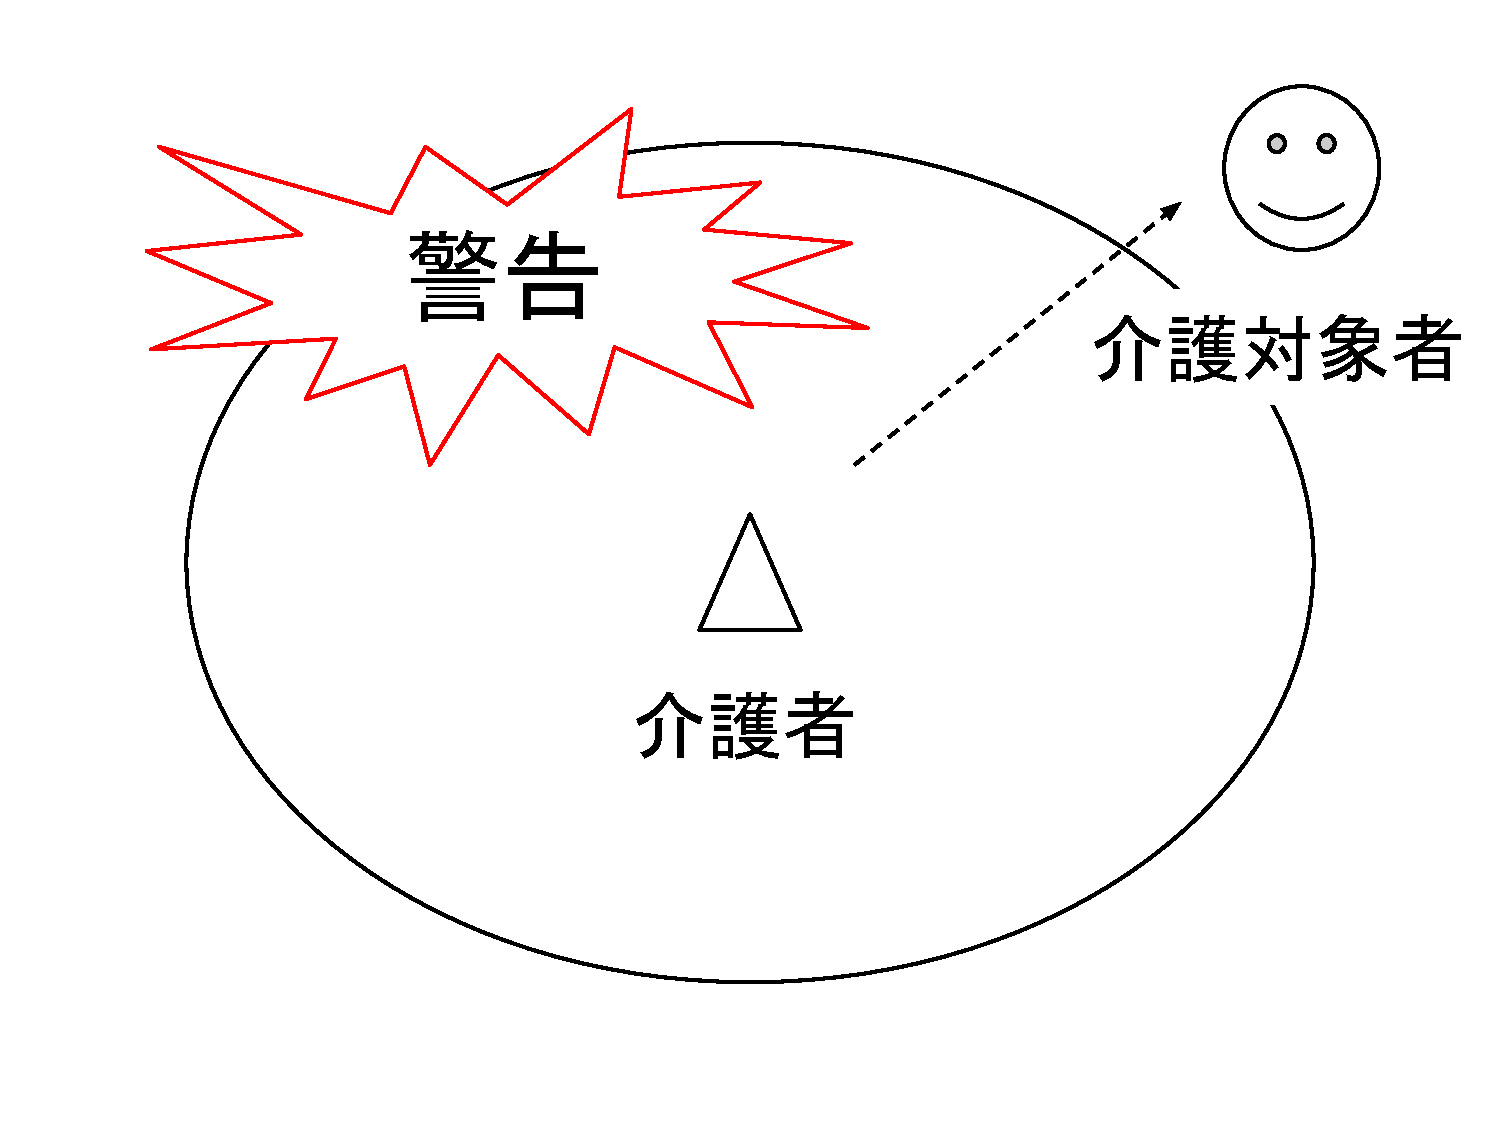
\includegraphics[width=10cm]{fig/deviation.pdf}
\caption{見守りエリアからの逸脱管理}
\end{figure}

\newpage

\section{ビーコン情報の共有}
受信用スマートフォンが複数ある場合は,スマートフォン同士で発信機の情報を共有し,見守りエリアを拡大させる.
自らの見守りエリアから逸脱した発信機が,他のスマートフォンで検知されていれば見守りは成功していると判断で
きる.
スマートフォン同士で共有する発信機の情報は,

\begin{itemize}
\item タイムスタンプ
\item 各自の見守りエリアにある発信機ID
\item 見守りエリアから逸脱した発信機ID
\end{itemize}

以上の三つである.これらの情報を共有することで,同じアドホックネットワーク内にある他のスマートフォンが検知している発信機を知ることができ,見守りエリアを拡大することができる.

\begin{figure}[htbp]
\centering
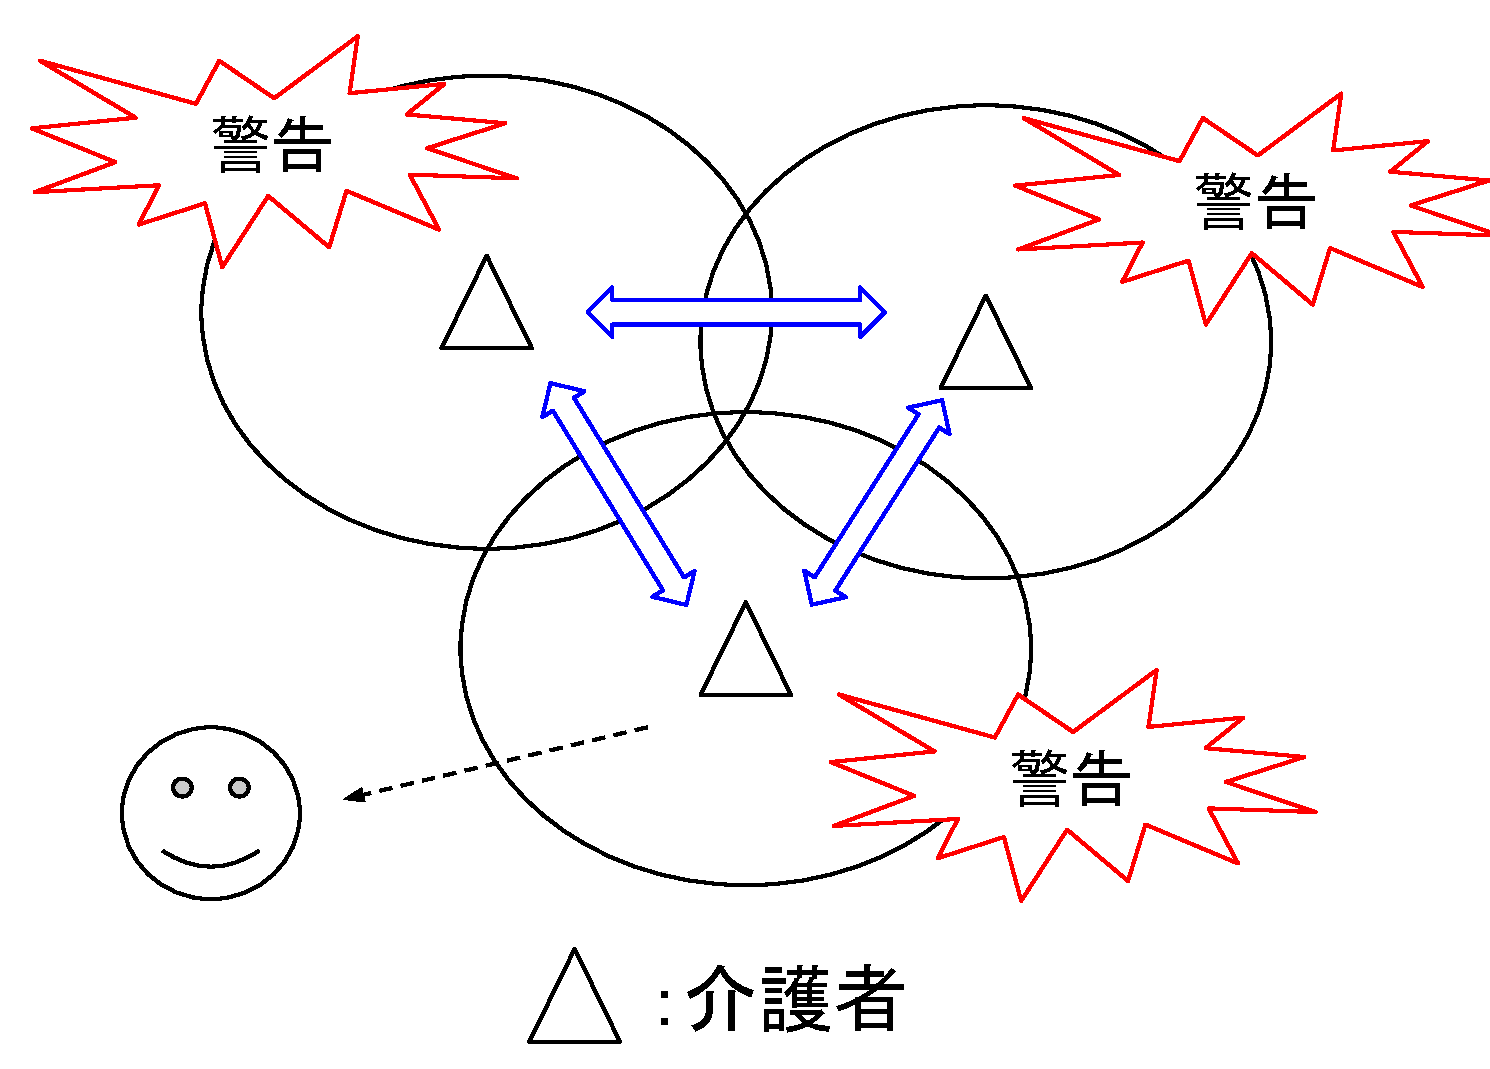
\includegraphics[width=10cm]{fig/share.pdf}
\caption{ビーコン情報の共有}
\end{figure}


%実験
\chapter{設計と実装}
\label{chap:poordirection}

\section{提案手法}
本研究では,P2P型端末通信フレームワークであるAllJoynを用いて端末間のビーコン情報共有を行う.
具体的には,端末Aで周囲のビーコンを検知し,端末BにビーコンのUUID,RSSIなどの情報を送信する.
また,自身で検知したビーコンの情報と,他端末から送信されたビーコンの情報を保持する.
今回の設計では,同一アクセスポイント内に全ての端末があることを想定している.

\section{開発環境}
本研究では,対象OSをAndroidとし,Android OSで動作するアプリケーションを作成する.
なお,Android 4.3以上かつBluetooth4.0以上に対応した端末を想定している.
\begin{itemize}
\item 開発環境
\begin{itemize}
\item Eclipse 3.8 for Mac OS X
\item Android SDK Tools 23.0.5
\item AllJoyn Android v14.02
\end{itemize}
\item 使用端末
\begin{itemize}
\item TORQUEG01
\item ARROWS NX F-05F
\end{itemize}
\end{itemize}

使用した端末のスペックは以下の通りである.
\begin{table}[htbp]
\centering
\begin{tabular}{|c|c|} \hline
OS &  4.4.2 \\ \hline
CPU & MSM8928 1.4GHz クアッドコア \\ \hline
ROM & 16GB \\ \hline
RAM & 2GB \\ \hline
Bluetooth & Ver.4.0 \\ \hline
Wi-Fi & IEEE802.11a/b/g/n/ac \\ \hline
\end{tabular}
\caption{スペック:TORQUE G01}
\end{table}

\begin{table}[htbp]
\centering
\begin{tabular}{|c|c|} \hline
OS &  4.4.2 \\ \hline
CPU & MSM8974 2.3GHz クアッドコア \\ \hline
ROM & 32GB \\ \hline
RAM & 2GB \\ \hline
Bluetooth & Ver.4.0 \\ \hline
Wi-Fi & IEEE802.11a/b/g/n/ac \\ \hline
\end{tabular}
\caption{スペック:ARROWS NX F-05F}
\end{table}


\section{AllJoynAppの概要}
iBeaconから発せられるビーコンを受信し,AllJoynを用いてビーコン情報を送受信するAndroidアプリであるAllJoynAppを作成する.


\subsection{設計}
今回作成するAllJoynAppには,ビーコンを検知し,AllJoynを用いてビーコン情報を送信するAllJoynClientと,ビーコン情報を受信するAllJoynService,インターフェースを記述したSimpleInterfaceという三つのプログラムがある.
AllJoynServiceはバックグラウンドで動作するプログラムであり,AllJoynClientから呼び出されて起動する.
更に,FINDボタンとSCANボタン,ListViewといったUI部品がある.


\subsection{AllJoynセッション}
今回設計したAllJoynAppのセッションの流れは以下の通りである.

\begin{figure}[htbp]
\centering
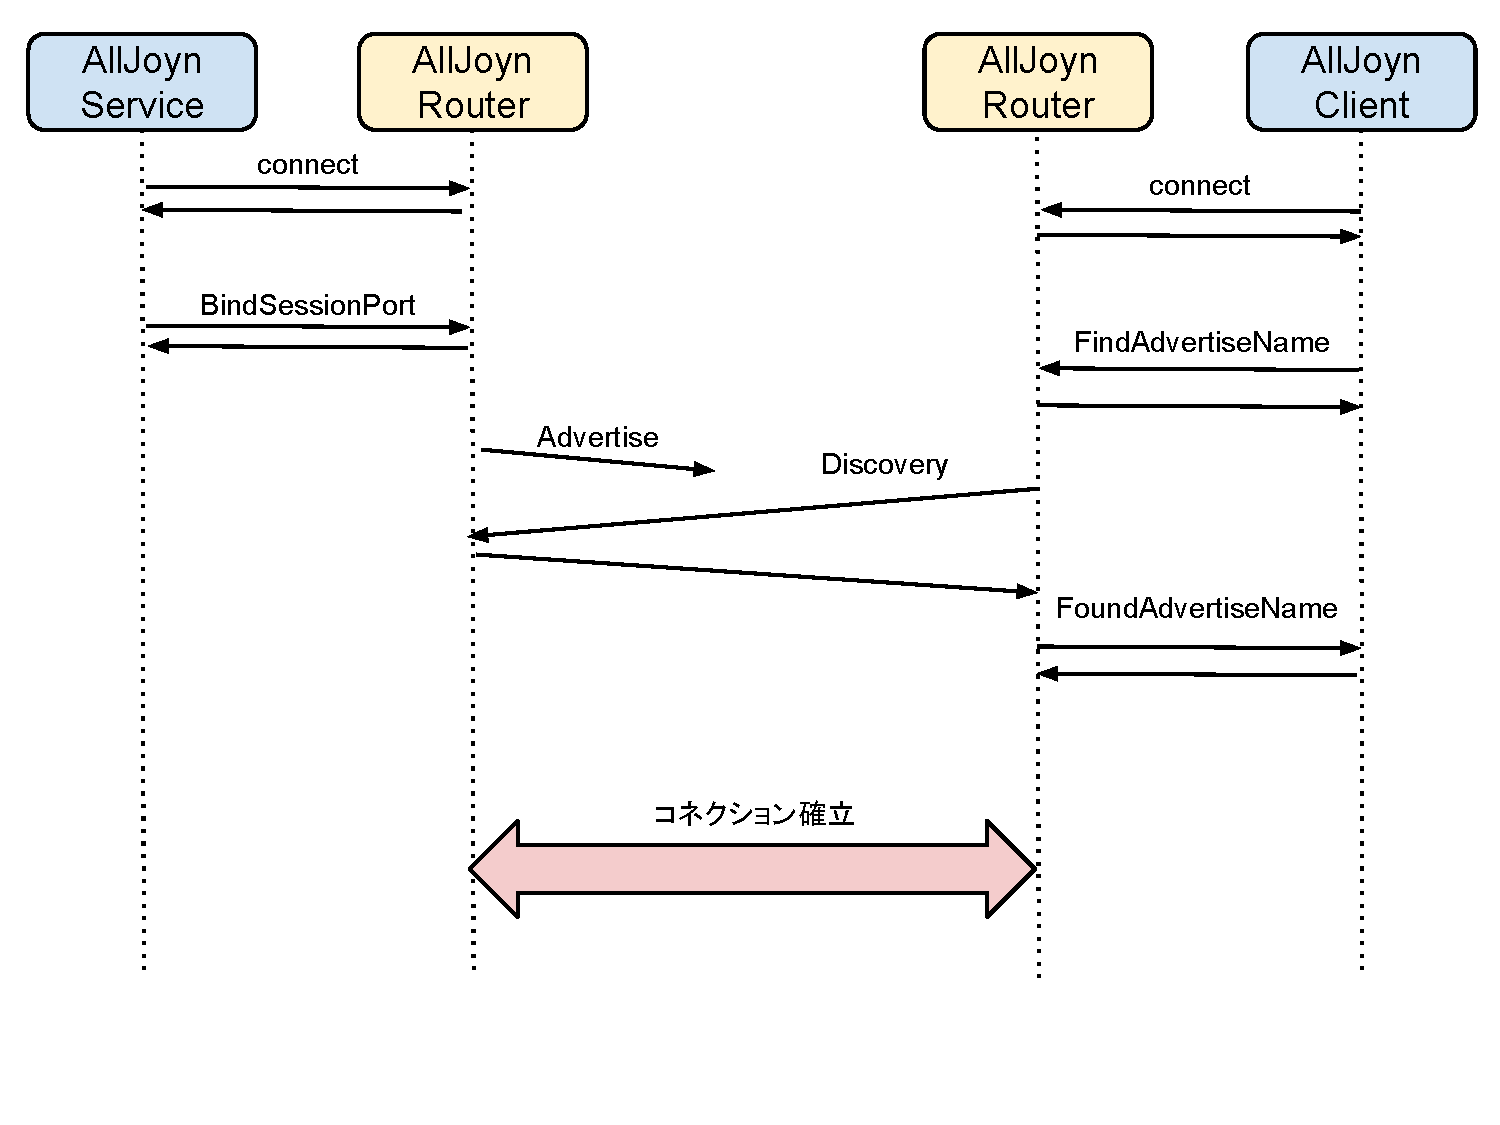
\includegraphics[width=10cm]{fig/AllJoyn_Session.pdf}
\caption{AllJoynセッションの例}
\end{figure}

\begin{enumerate}
\item AllClientとAllJoynServiceは,それぞれのAllJoyn Routerに接続する.
\item AllJoynServiceでは,BindSessionPort APIを用いてセッションポートやセッションオプションなどを決定する.
\item AllJoynServiceでは,AllJoyn Routerを通して任意の名前をAdvertiseしてコネクションを待つ.
\item AllJoynClientでは,AllJoyn Routerを通して任意の名前をDiscoverする.
\item Advertiseされている任意の名前と一致した場合,FoundAdvertiseNameシグナルがAllJoynClientに送られる.
\item AllJoynClientがJoinSession APIを用いてAllJoynClientとAllJoynServiceのコネクションが確立する.
\end{enumerate}


\subsection{iBeaconの検知}
iBeaconはiOS特有の機能であるが,Bluetooth Low Energy(BLE)を利用した技術であるため,BLEを受信することができるAndroid4.3以上かつBluetooth4.0に対応した端末ならiBeaconを検知することができる.
iBeaconがブロードキャストしているバイトデータは6$\sim$9バイト目が固定されており,この値を参照してiBeaconかどうかを判断する.

\begin{table}[htbp]
  \centering
  \begin{tabular}{|c|c|} \hline
    データ領域 & 説明 \\ \hline \hline
    1   & 1ブロック目のバイト数 \\ \hline
    2,3 & フラグ \\ \hline
    4   & 2ブロック目のバイト数 \\ \hline
    5   & メーカー固有のAD typeデータ \\ \hline
    6,7 & 会社コード(Appleのコードは0x004C) \\ \hline
    8   & データタイプ(iBeaconは0x02) \\ \hline
    9   & 連なるiBeaconデータのバイト数 \\ \hline
    10 $\sim$ 25 & UUID \\ \hline
    26,27 & major \\ \hline
    28,29 & minor \\ \hline
    30  & 受信強度を求めるための2の補数 \\ \hline
  \end{tabular}
  \caption{iBeaconデータ配列}
\end{table}

Androidアプリ内でバイトデータを処理し,UUIDやrssiといったビーコン情報を抽出する.


\subsection{プログラムファイル}
AllJoynAppは,
\begin{itemize}
\item AllJoynClient.java
\item AllJoynService.java
\item SimpleInterface.java
\end{itemize}
の三つのプログラムファイルから成る.


\begin{figure}[htbp]
\begin{center}
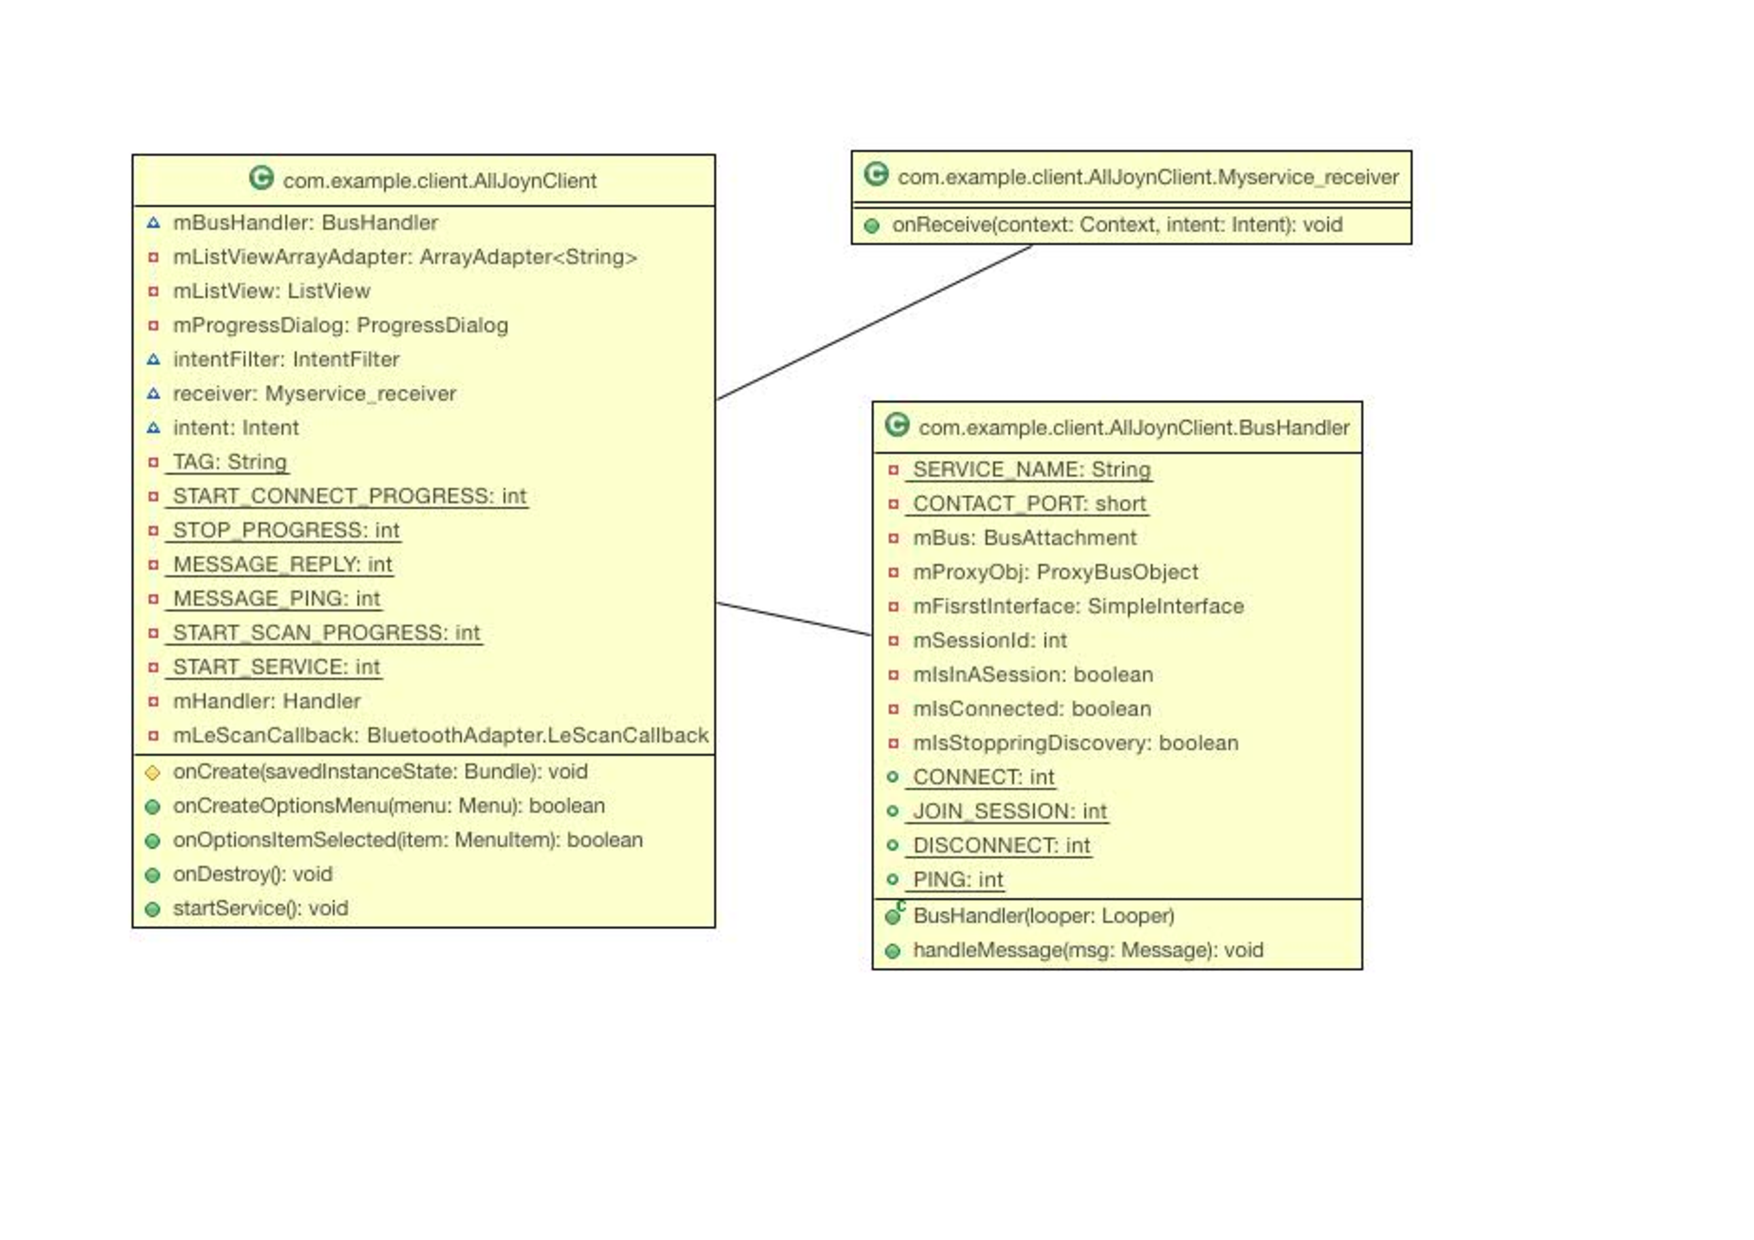
\includegraphics[width=10cm]{fig/class_client.pdf}
\end{center}
\caption{AllJoynClientクラス図}
\end{figure}

\begin{figure}
\begin{center}
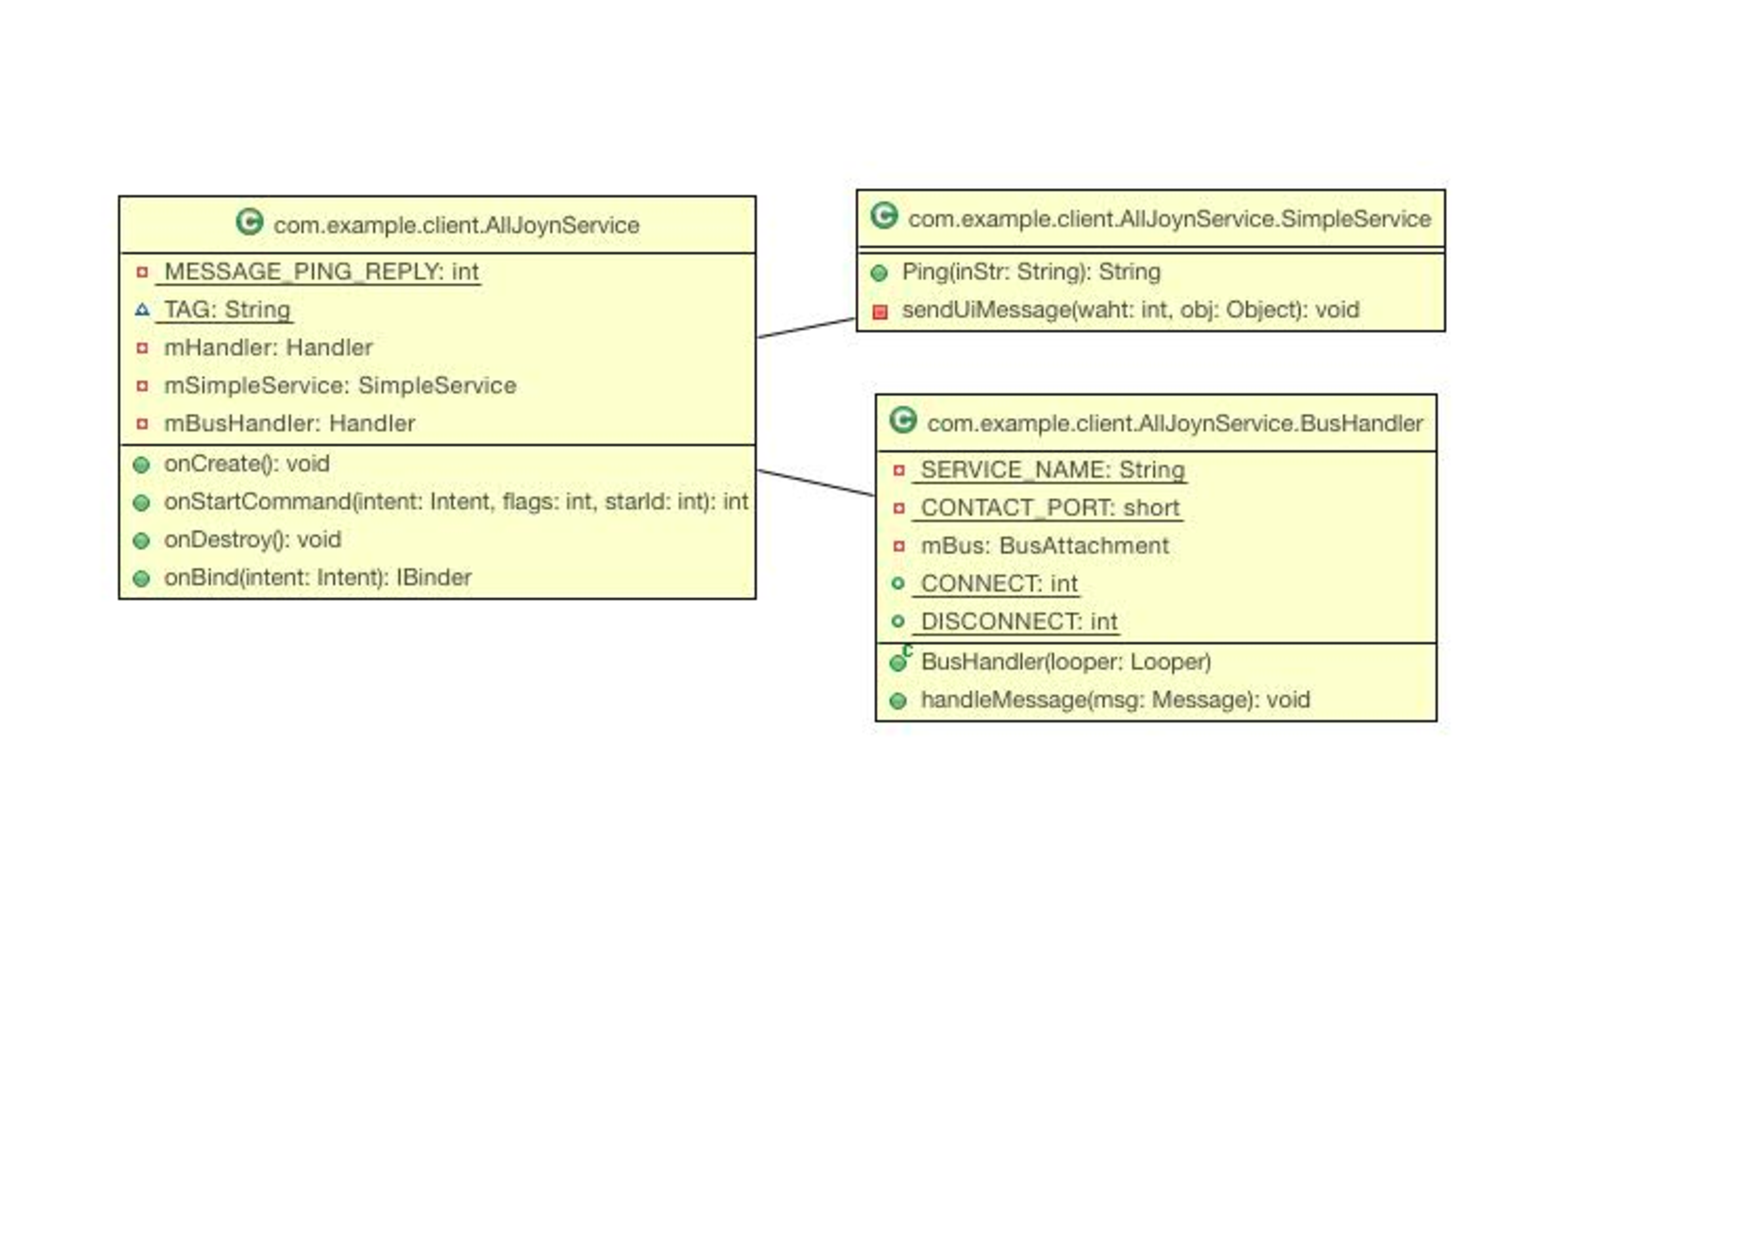
\includegraphics[width=10cm]{fig/class_service.pdf}
\end{center}
\caption{AllJoynServiceクラス図}
\end{figure}

\begin{figure}[htbp]
\centering
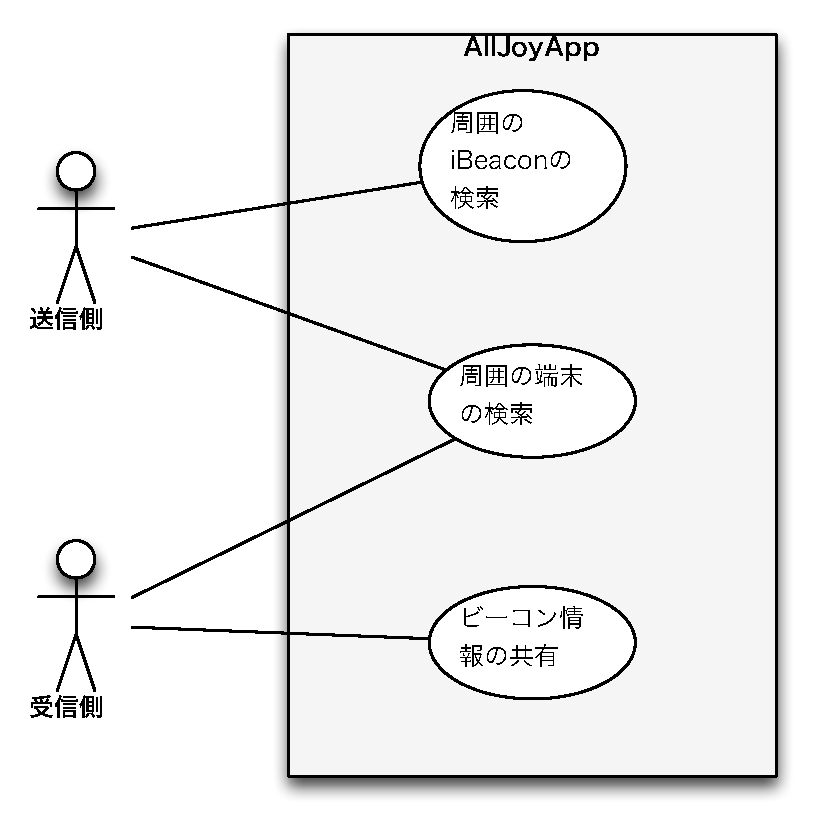
\includegraphics[width=7cm]{fig/usecase.pdf}
\caption{ユースケース図}
\end{figure}

\section{実装}
今回作成したAllJoynAppの処理を解説する.
操作の手順としては
\begin{enumerate}
\item アプリケーションの起動
\item FINDボタン押下
\item SCANボタン押下
\end{enumerate}
となっている.

\subsection{アプリケーションの起動}
アプリケーションを起動した際の処理は以下の通りである.

\begin{enumerate}
\item AllJoynClientを起動する.
\item AllJoynClientはAllJoynServiceを起動する.AllJoynServiceはバックグラウンドで動作する.
\item 画面上にFIND,SCANという二つのボタンを表示する.
\item AllJoynServiceはAllJoyn Routerと接続し,Advertiseする.
\end{enumerate}

\begin{figure}[htbp]
\centering
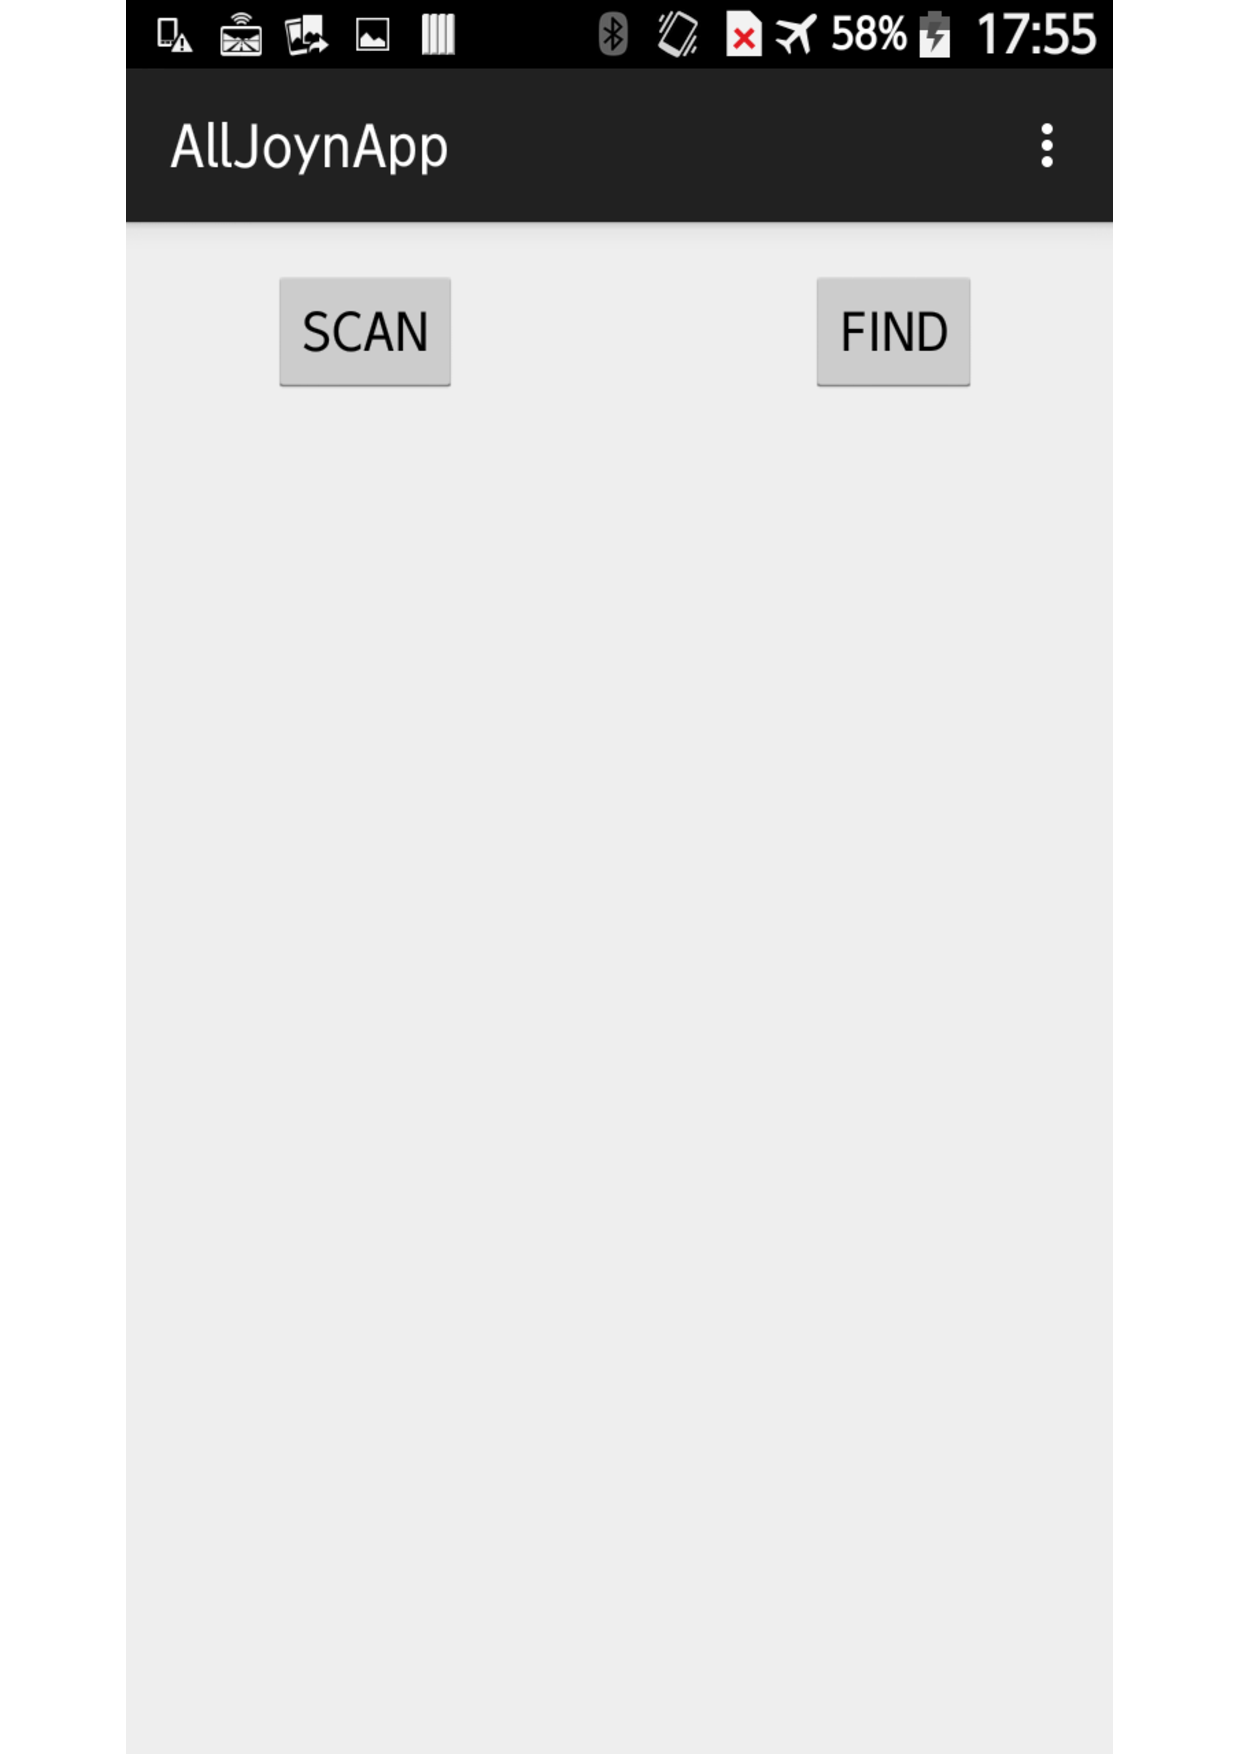
\includegraphics[width=5cm]{fig/screen1.pdf}
\caption{アプリケーション起動画面}
\end{figure}

以下の図は,端末A,端末BでAllJoynAppを起動した様子を表している.
端末A及び端末Bでは,AllJoynServiceが起動し,周囲にAdvertisementしている.

\begin{figure}[htbp]
\centering
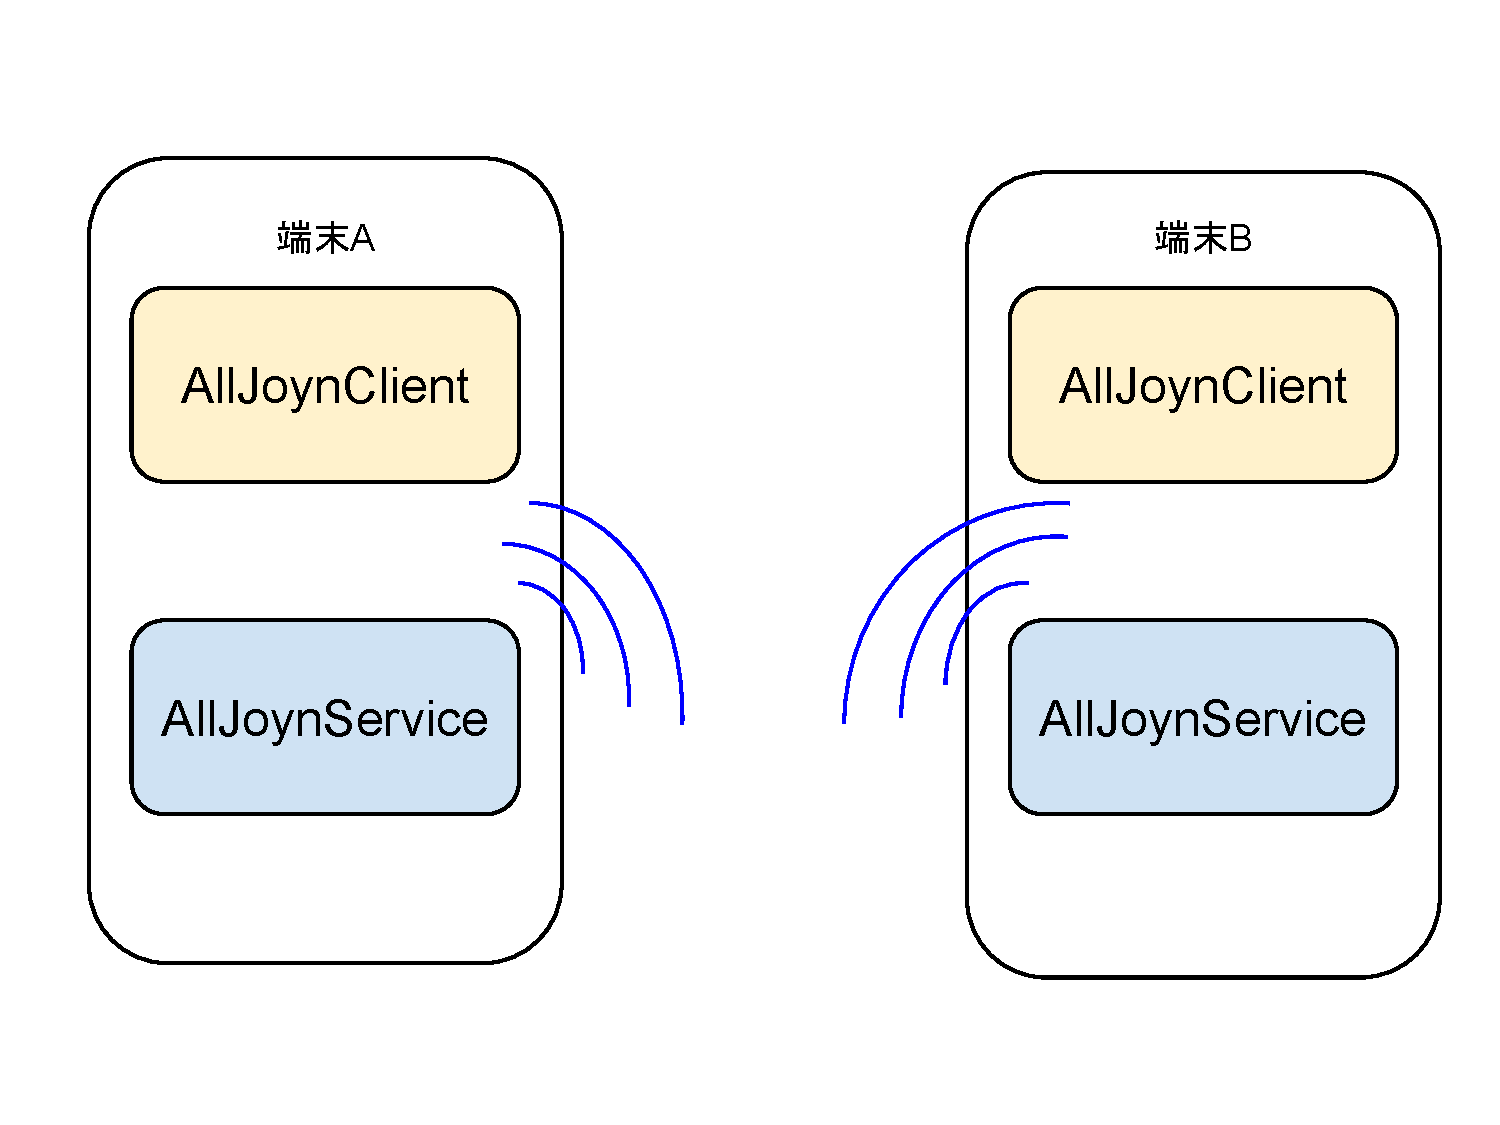
\includegraphics[width=10cm]{fig/appstart.pdf}
\caption{アプリケーション起動画面}
\end{figure}



\subsection{FINDボタン押下}
FINDボタンを押下した際の処理は以下の通りである.

\begin{enumerate}
\item 自身のAllJoynServiceを停止する.
\item AllJoynClientは自身のAllJoynRouterと接続する
\item 周囲のAllJoynServiceをDiscoveryする.
\item 検索している間,画面上には'DISCOVERING'と表示される
\item AllJoynServiceを検知した場合,コネクションを確立し,'DISCOVERING'の表示をやめる.
\end{enumerate}

同端末内でAllJoynClientとAllJoynServiceが起動している際,AllJoynClientは自身のAllJoynServiceと優先的に接続するため,Discoveryする前に自身のAllJoynServiceを停止させて周囲のAllJoynServiceをDiscoveryする.

\begin{figure}[htbp]
\centering
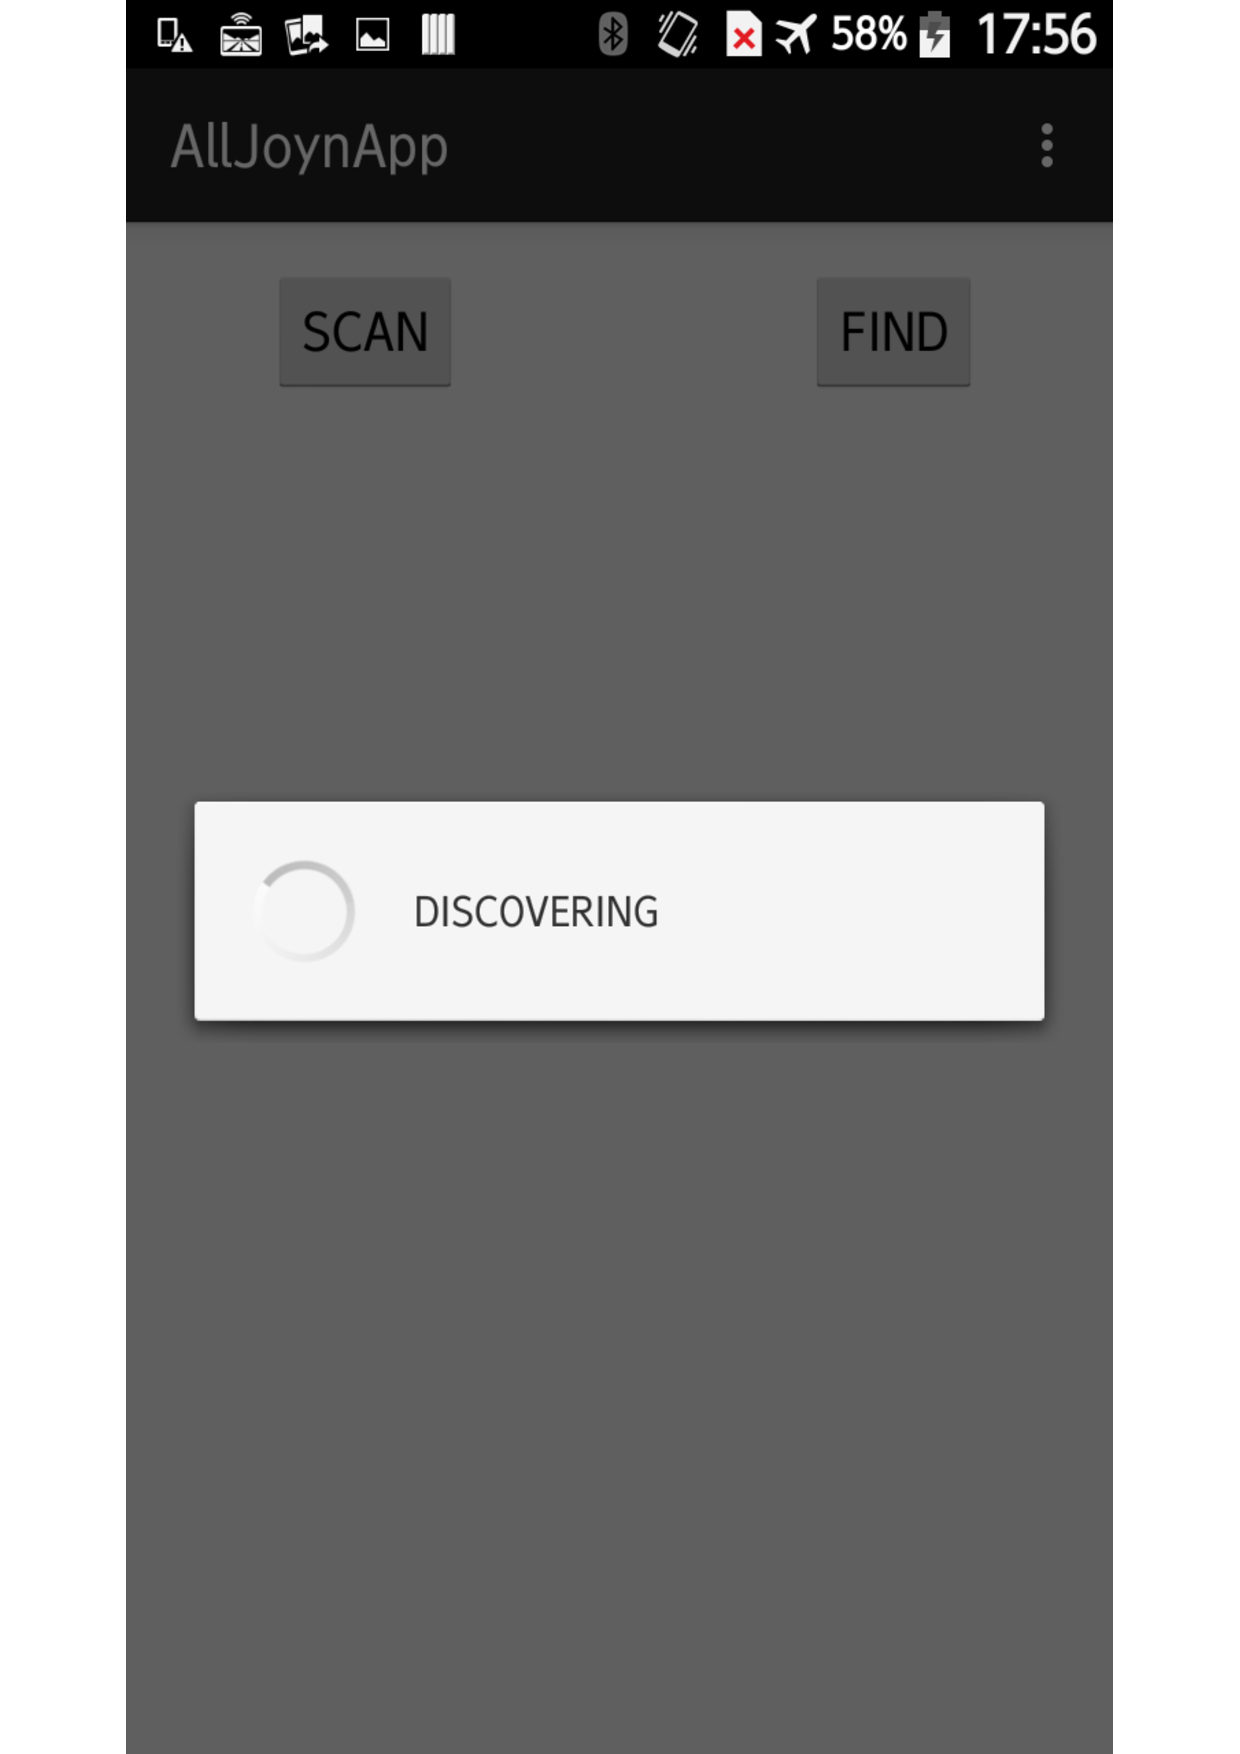
\includegraphics[width=5cm]{fig/screen2.pdf}
\caption{FINDボタン押下}
\end{figure}

以下の図では,端末AでFINDボタンを押下した際の様子を表している.
端末AではAllJoynServiceが停止し,端末AのAllJoynClientは端末BのAllJoynServiceとコネクションを確立させる.

\begin{figure}[htbp]
\centering
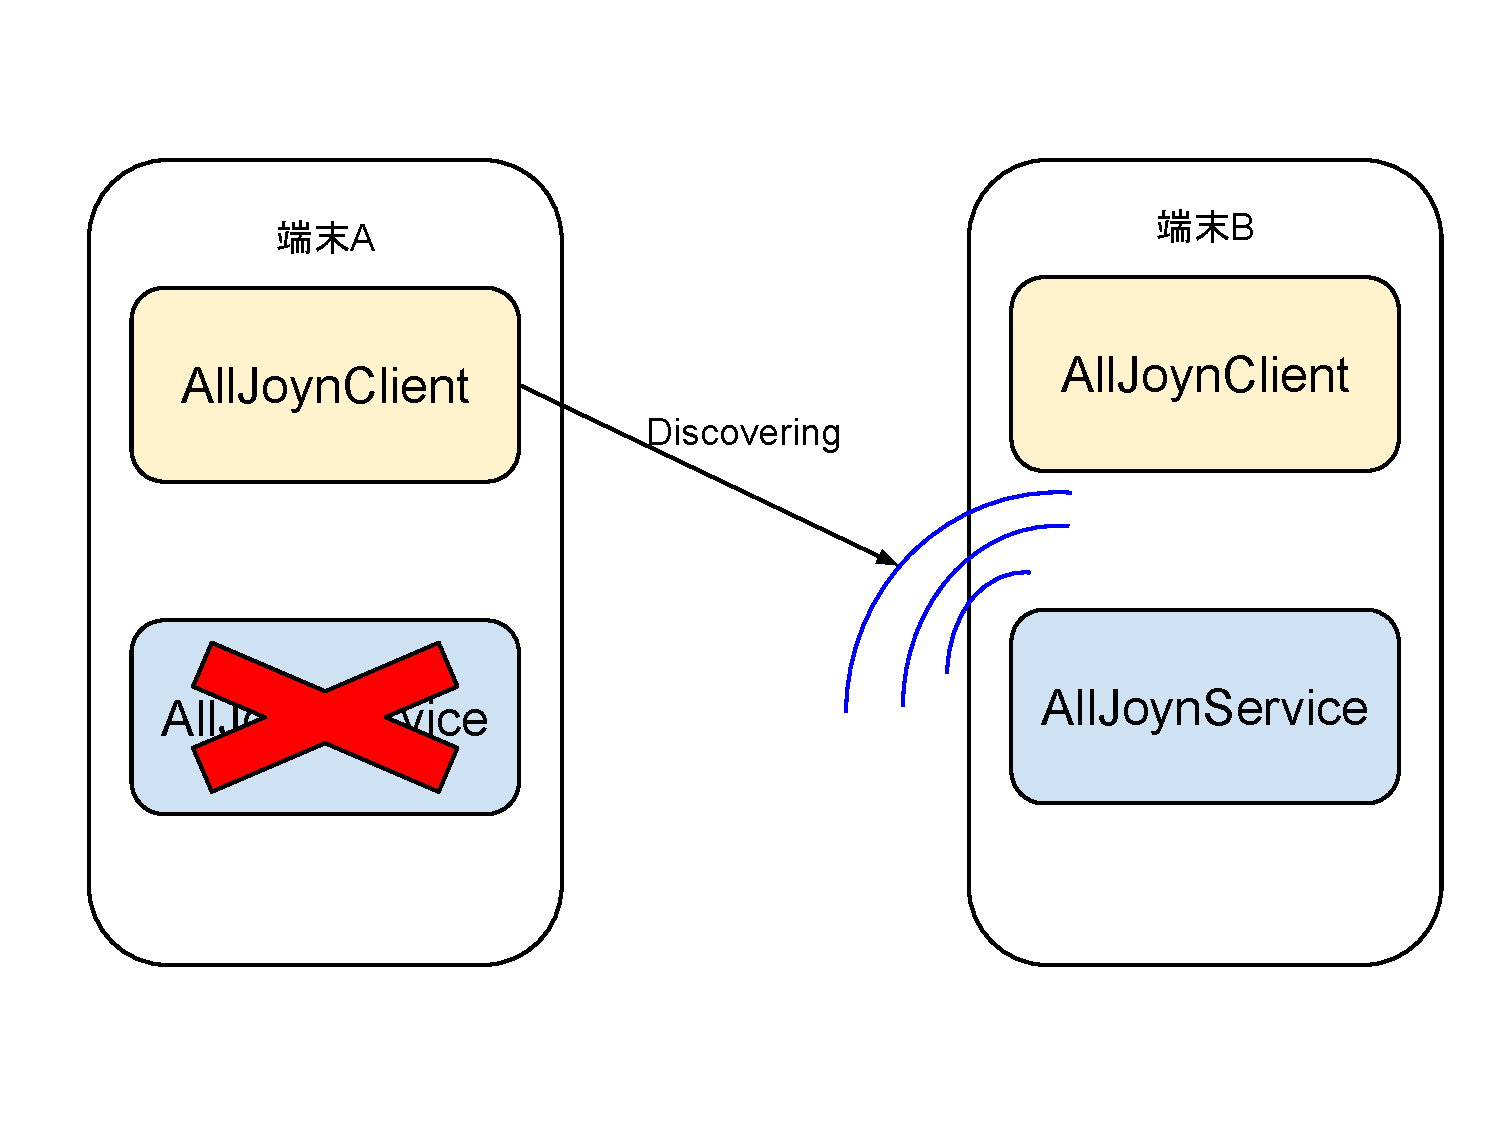
\includegraphics[width=10cm]{fig/click_find.pdf}
\caption{FINDボタン押下}
\end{figure}

\newpage

\subsection{SCANボタン押下}
SCANボタンが押下された際の処理は以下の通りである.
\begin{enumerate}
\item 二秒間周囲のiBeaconを検知し,ビーコン情報を画面上に表示する.iBeaconを検知しなかった場合,画面上に'iBeacon not found'と表示する.
\item AllJoynClientから,接続しているAllJoynServiceにビーコン情報を送信する.
\item ビーコン情報を受信したAllJoynServiceは,自身のAllJoynClientにビーコン情報を送信する.
\item AllJoynClientは,受信したビーコン情報を画面上に表示する.
\item 自身のAllJoynServiceを起動する.
\end{enumerate}


\begin{figure}[htbp]
\centering
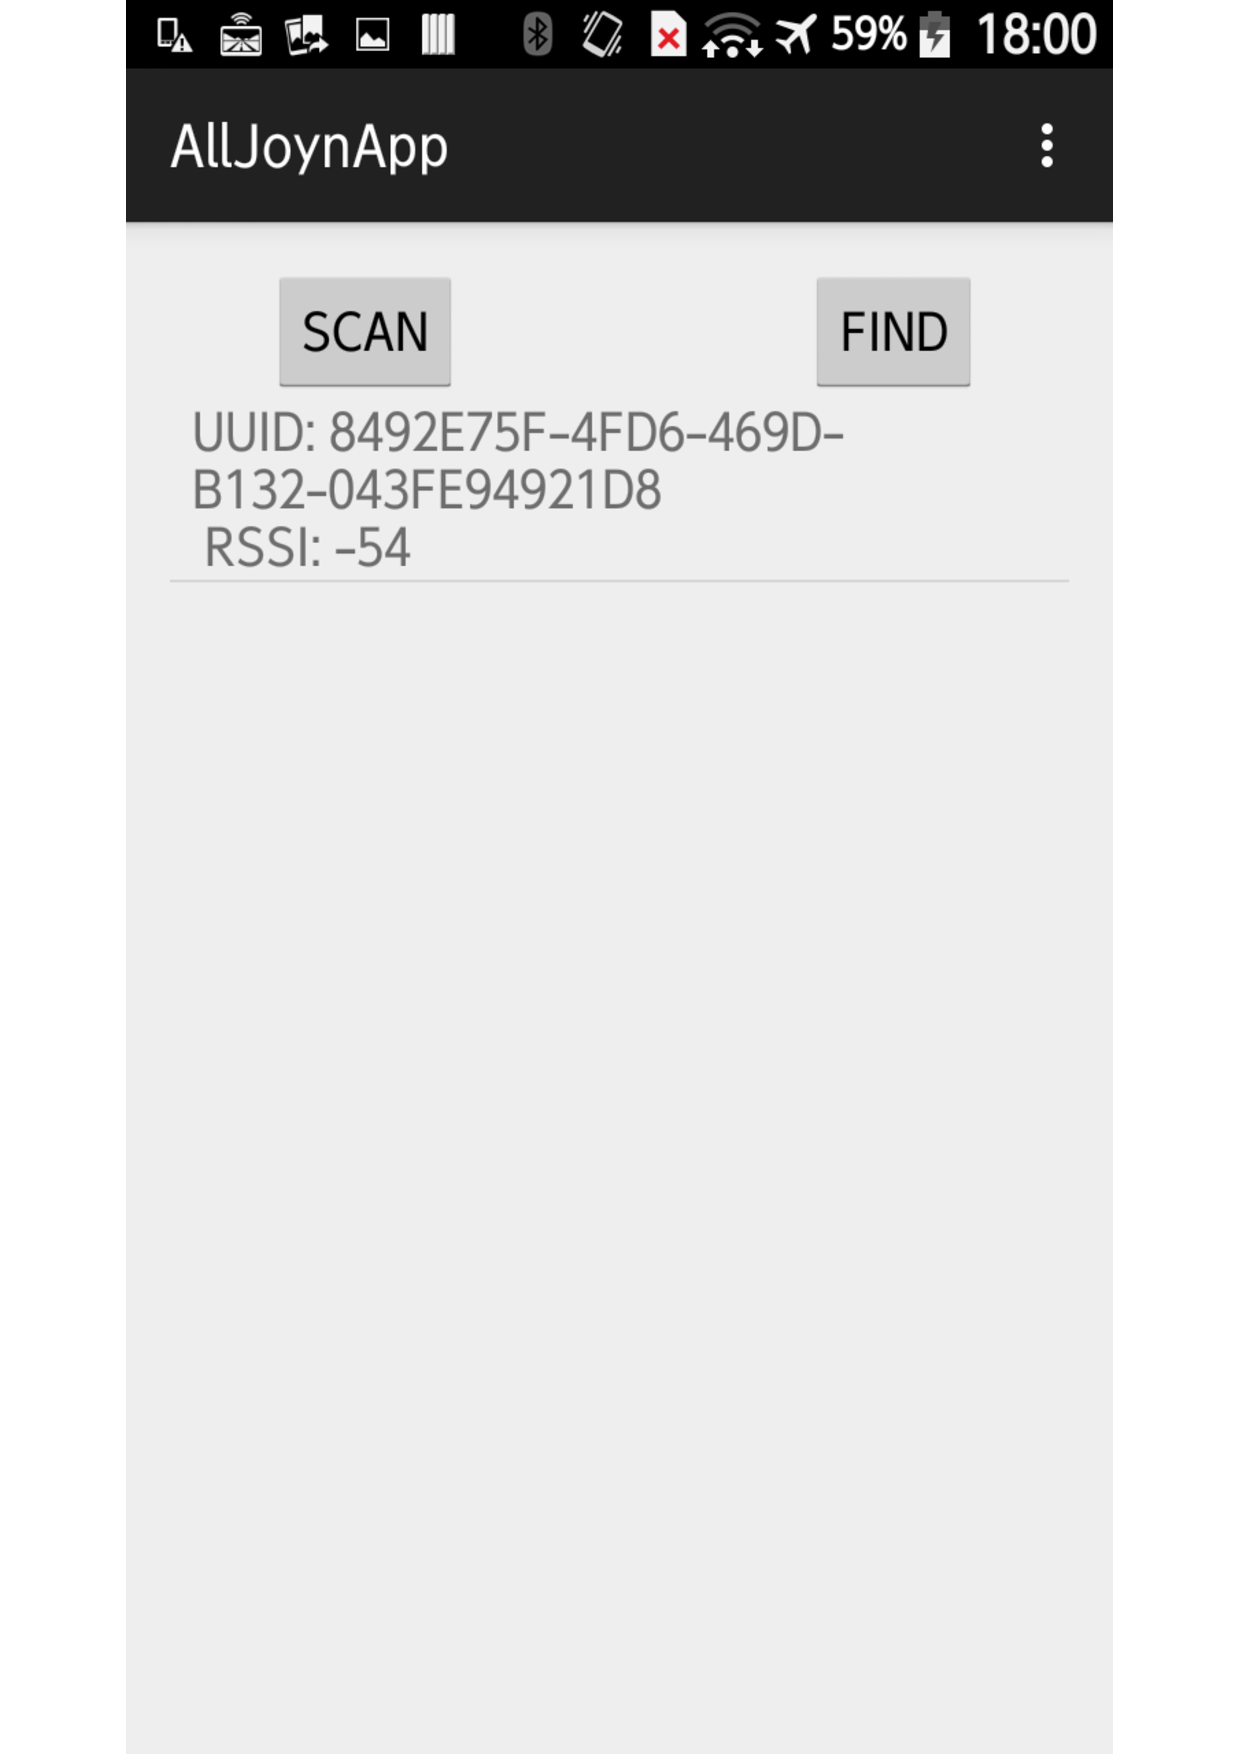
\includegraphics[width=5cm]{fig/screen3.pdf}
\caption{SCANボタン押下}
\end{figure}

以下の図は端末AでSCANボタンを押下した際の様子を表している.
端末AのAllJoynClientでビーコンを検知し,端末BのAllJoynServiceにビーコン情報を送信する.端末BのAllJoynServiceは自身のAllJoynClientにビーコン情報を送信し,画面上に表示する.

\begin{figure}[htbp]
\centering
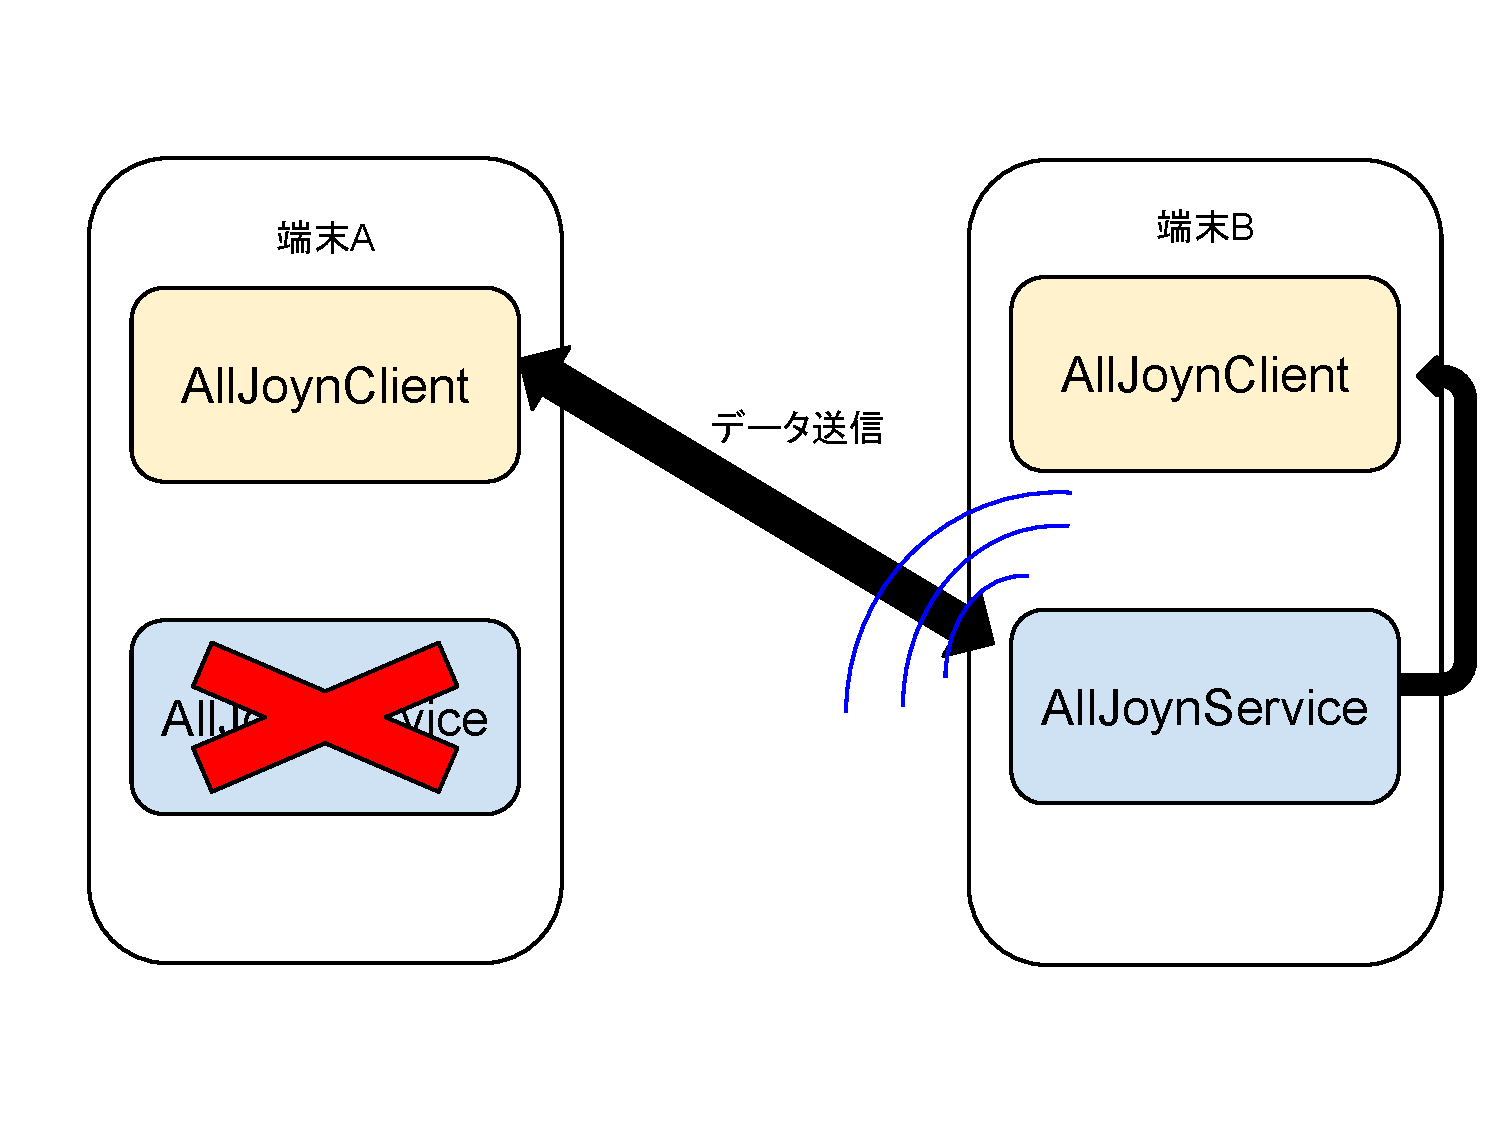
\includegraphics[width=10cm]{fig/click_scan.pdf}
\caption{SCANボタン押下}
\end{figure}






% 今後の課題
\chapter{結論}
\section{結論}
本研究では,スマートフォン同士のアドホックネットワークの構築と,情報共有手法の実装を目的とした.
検証の結果から,情報共有手法の実装という目的は達成できたといえるが,アドホックネットワークの構築は達成することができなかった.

\section{今後の課題}
検証で得られたデータから,現在のアプリケーションに追加すべき機能や改善点を検討する.

\begin{itemize}
\item アドホックネットワーク \\
スマートフォン同士でのアドホックネットワークを構築し,屋外での見守りにも対応する必要がある.
そのためには,AllJoyn使用環境の検証やAllJoynの拡張をしていく必要があると考えられる.

また,今回の検証では機材の関係上端末二台での通信だったが,端末の数を増やした場合の検証をしていく必要がある.

\item 情報共有手法 \\
今回の設計では,端末が二台しかないという関係上,二台間での情報共有に留まっている.
そのため今後,端末が三台以上での情報共有を想定し設計・実装をしなければならない.

\item アプリケーション全般 \\
  周囲にあるiBeaconを全て検知するという設計で開発を行ったが,実際の利用を想定した場合,アプリケーションの画面から検知するiBeaconを指定することができるようにする必要がある.
  
  また,DiscoveryやiBeaconのスキャンの処理をボタンを押下することによって開始しているが,ユーザーが操作することなく自動で処理を開始するよう設計する必要がある.
  
  ビーコン情報の共有に注力してアプリケーションを作成したため,UI部分が洗練されていない.
今後,より検証を重ねてUIを洗練させていく必要がある.

\item 検証 \\
端末やiBeacon発信機の数を更に増やして,検知できるiBeaconの数などの検証を進めていく必要がある.
また,実際の利用環境での検証や長期間の運用実験を行い,データを収集するべきである.


\end{itemize}





% 参考文献
% 参考文献
\def\line{−\hspace*{-.7zw}−}

\begin{thebibliography}{99}
%\bibitem{*}内の * は各自わかりやすい名前などをつけて、
%論文中には \cite{*} のように使用する。
%これをベースに書き換えた方が楽かも。
%書籍、論文、URLによって若干書き方が異なる。
%URLを載せる人は参考にした年月日を最後に記入すること。


\bibitem{hoge}
hoge
\end{thebibliography}


% 謝辞
\chapter*{謝辞}
\thispagestyle{empty}

%基本的な内容は以下の通り.参考にしてみて下さい.
%厳密な決まりは無いので,個々人の文体でも構わない.
%GISゼミや英語ゼミに参加した人はその分も入れておく.
%順番は重要なので気を付けるように.(提出前に周りの人に確認してもらう.)

\hspace{1zw}本研究の遂行,また本論文の作成にあたり,御多忙にも関わらず終始懇切なる御指導と御教授を賜わりました宮里智樹助教に深く感謝したします.

また,本研究の遂行及び本論文の作成にあたり,御教授と御指導を賜りました宮里研究室の早乙女さん,桃原さん,花城さんに感謝します.

また一年間共に研究を行い、暖かな気遣いと励ましをもって支えてくれた宮里研究室の饒平名長太君、呉屋桂基君に感謝します.

また,有意義な時間を共に過ごした情報工学科の学友、並びに物心両面で支えてくれた両親に深く感謝致します。



\begin{flushright}
2月18日 新里亮太
\end{flushright}




% 付録
%\input{appendix.tex}

\end{document}
